
\documentclass[xcolor=dvipsnames]{beamer}
\usepackage{lmodern}
\usepackage[T1]{fontenc}
\usepackage{graphicx}
\usepackage{ucs}
\usepackage[utf8x]{inputenc}
\setbeamertemplate{items}[ball]
\setbeamertemplate{blocks}[rounded][shadow=true]
\setbeamertemplate{navigation symbols}{}
\usecolortheme[named=Apricot]{structure}
\useoutertheme{infolines}
\author{Jonathan Poelen, Christophe Grosjean}
\institute{Wallix}
\title{OCR}
\usetheme{Madrid}
\usepackage{tikz}
\usetikzlibrary{shapes.geometric}
\usepackage{tikz}
\usepackage{tikz}
\usetikzlibrary{arrows,shadows} % for pgf-umlsd
\usepackage[underline=true,rounded corners=false]{pgf-umlsd}
\usepackage{pgf-umlsd}
\usepackage{listings}
\usepackage{svg}
\usepackage{amsmath}

%\graphicspath{{illustrations/}}

\begin{document}
\begin{frame}[plain]
\titlepage
\end{frame}


\begin{frame}
\frametitle{l'OCR dans le WAB: pour quoi faire ?}
    \setbeamercolor{block body alerted}{fg=white,bg=blue}
    \begin{center}
       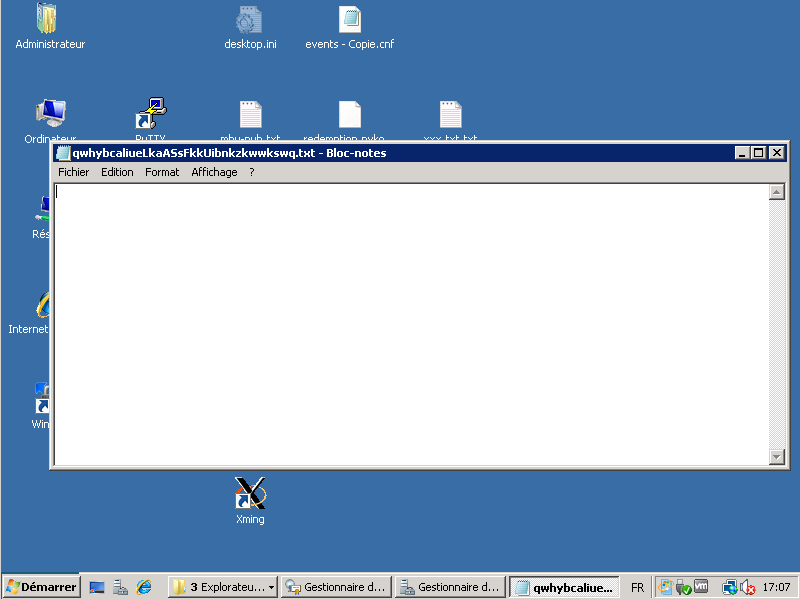
\includegraphics[width=200px]{TBar2.png}
      \begin{alertblock}{}
            \begin{center}
                  \textbf{\Large Détecter les textes des barres de titre des applications Windows}
            \end{center}
      \end{alertblock}
    \end{center}
\end{frame}

\begin{frame}
\frametitle{l'OCR dans le WAB: pour quoi faire ?}
    \setbeamercolor{block body alerted}{fg=white,bg=blue}
    \begin{center}
       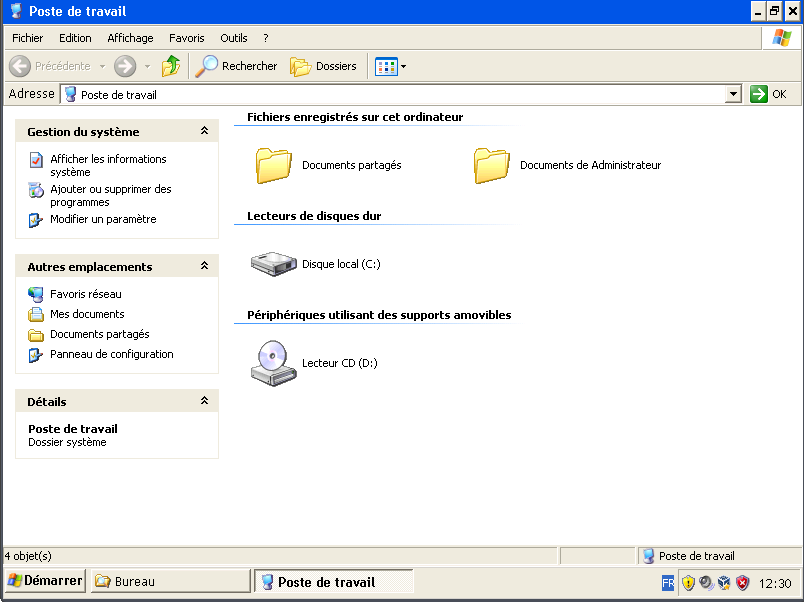
\includegraphics[width=200px]{PosteDeTravail.png}
      \begin{alertblock}{}
            \begin{center}
                  \textbf{\Large Mais elles peuvent aussi ressembler à ça}
            \end{center}
      \end{alertblock}
    \end{center}
\end{frame}

\begin{frame}
\frametitle{l'OCR dans le WAB: pour quoi faire ?}
    \setbeamercolor{block body alerted}{fg=white,bg=blue}
    \begin{center}
       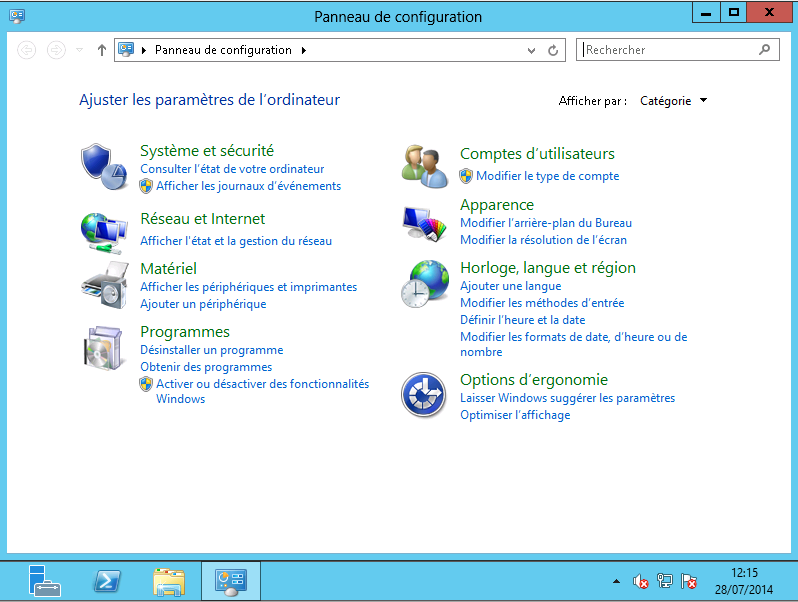
\includegraphics[width=200px]{TBar1.png}
      \begin{alertblock}{}
            \begin{center}
                  \textbf{\Large ou à ça}
            \end{center}
      \end{alertblock}
    \end{center}
\end{frame}

\begin{frame}
\frametitle{l'OCR dans le WAB: pour quoi faire ?}
    \setbeamercolor{block body alerted}{fg=white,bg=blue}
    \begin{center}
       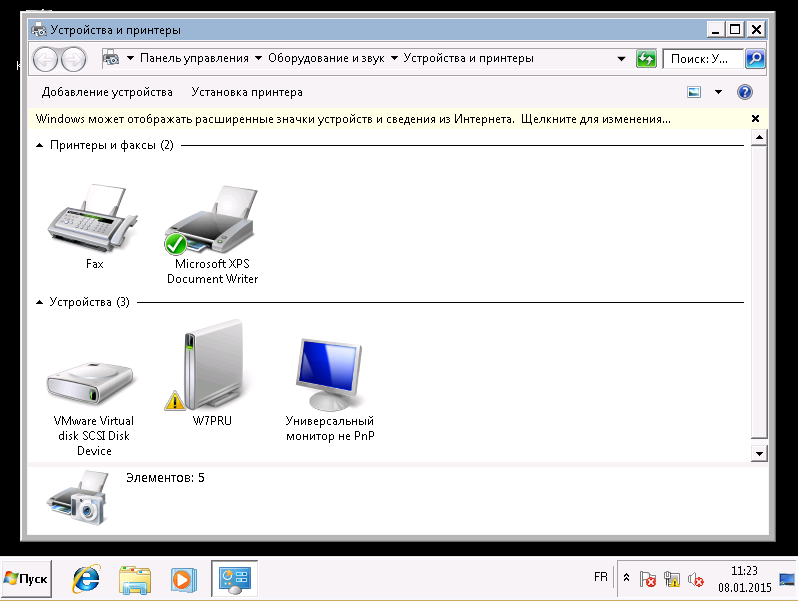
\includegraphics[width=200px]{TBar3.png}
      \begin{alertblock}{}
            \begin{center}
                  \textbf{\Large ou encore à ça}
            \end{center}
      \end{alertblock}
    \end{center}
\end{frame}

\begin{frame}
\frametitle{OCR: solution actuelle}
    \begin{itemize}
    \item Localiser les barres de titre dans l'image (à partir de la couleur de fond)
    \item une fois la barre de titre repérée isoler chaque lettre par un balyage horizontal
    \item la reconnaîssance du texte dans les barres de titre se base sur les pixels exacts des polices reconnues
    \item on ne regarde même pas tous les pixels, juste ceux nécessaires pour différencier les lettres
    \end{itemize}
\end{frame}

\begin{frame}
\frametitle{OCR: solution actuelle}
    \setbeamercolor{block body alerted}{fg=white,bg=blue}
    \begin{center}\begin{alertblock}{}
            \begin{center}\textbf{\Large Avantages}\end{center}
    \end{alertblock}\end{center}
    \begin{itemize}
    \item très rapide: > 1000 barres de titre par seconde
    \item code pas trop compliqué (après gros nettoyage pour enlever Milena)
    \item code maitrisé, on peut ajouter ou enlever des polices, 
    \item supporte désormais les caractères cyrilliques
    \end{itemize}
    \begin{center}\begin{alertblock}{}
            \begin{center}\textbf{\Large Inconvénients}\end{center}
    \end{alertblock}\end{center}
    \begin{itemize}
    \item faux positifs
    \item ne marche pas sur des polices inconnues (même ressemblantes)
    \item ne marche pas sur des polices de taille différente
    \item problèmes avec le lissage et l'anti-aliasing (débrayable en RDP... mais pas complètement)
    \item problème avec les caractères collés (ligatures)
    \end{itemize}
\end{frame}

\begin{frame}
\frametitle{Utiliser un OCR du marché}
    \setbeamercolor{block body alerted}{fg=white,bg=blue}
    \begin{center}\begin{alertblock}{}
            \textbf{\Large Contraintes}
        \begin{itemize}
        \item Logiciels Libres
        \item sous Linux
        \item actif et maintenus        
        \item bonne qualité de reconnaissance
        \item rapide
        \item configurable, on voudrait pouvoir fournir des polices de référence
        \item simple
        \item intégrables sous forme de librairie
        \item juste la partie reconnaissance de caractères, on a pas besoin du reste
        \item et solide, faudrait pas que ça plante ou qu'il y ait des fuites mémoire
        \end{itemize}
    \end{alertblock}\end{center}
    \setbeamercolor{block body alerted}{fg=white,bg=red}
    \begin{center}\begin{alertblock}{}
            \begin{center}\textbf{\Large On ne serait pas un peu exigeant...}\end{center}
    \end{alertblock}\end{center}
\end{frame}


\begin{frame}
\frametitle{Utiliser un OCR du marché}
    \setbeamercolor{block body alerted}{fg=white,bg=blue}
    \begin{center}\begin{alertblock}{}
            \textbf{\Large Les candidats}
        \begin{itemize}
        \item Omnipage Pro SDK 19: Windows, KO
        \item PaperPort SDK: Windows, KO
        \item ABBYY Finereader Engine 11 SDK: Linux, Propriétaire, peut-être ?
        \item Tesseract: Libre, Linux, bonne qualité, à voir
        \item gOCR : Libre, Linux, bonne qualité, à voir
        \item Ocropus : Libre, Linux, reconnaissance pas terrible, KO
        \item OCrad : Libre, Linux, projet arrêté, KO
        \item Cuneiform : Libre, Linux, projet arrêté, KO
        \end{itemize}
    \end{alertblock}\end{center}
\end{frame}

\begin{frame}
\frametitle{Utiliser un OCR du marché : Tesseract}
    \setbeamercolor{block body alerted}{fg=white,bg=blue}
    \begin{center}\begin{alertblock}{}
            \textbf{\Large Avantages}
        \begin{itemize}
        \item projet leader en libre
        \item projet soutenu par google (pour leur numérisation massive de livres)
        \item bonne qualité de reconnaissance <5\% de caractères mal reconnus
        \item on peut l'alimenter avec des polices inconnues
        \item beaucoup de paramètres possibles (plusieurs centaines)
        \end{itemize}
    \end{alertblock}\end{center}
\end{frame}

\begin{frame}
\frametitle{Utiliser un OCR du marché : Tesseract}
    \setbeamercolor{block body alerted}{fg=white,bg=blue}
    \begin{center}\begin{alertblock}{}
            \textbf{\Large Inconvénients}
        \begin{itemize}
        \item trop de paramètres, complexes, parfois très impactants
        \item a du mal sur des polices < 12 pixels... dommage pour les titres
        \item (on peut grossir artificiellement les polices)
        \item optimisé pour des besoins qu'on a pas
        \begin{itemize}
        \item reconnaissance de livres scannés
        \item redresser le texte, antiparasite
        \item inutile pour de l'OCR écran
        \end{itemize}
        \item il y a surement la gestion de l'anti-aliasing quelque part... mais où?
        \item code très compliqués, passages de structures contenant à la fois les paramètres et les résultats
        \item code très gros : environ 200 000 lignes de C++
        \item très lent: de 3 à 5 barres de titre par seconde
        \item difficile à intégrer sous forme de librairie
        \end{itemize}
    \end{alertblock}\end{center}
\end{frame}

\begin{frame}
\frametitle{Utiliser un OCR du marché : gOCR}
    \setbeamercolor{block body alerted}{fg=white,bg=blue}
    \begin{center}\begin{alertblock}{}
            \textbf{\Large Avantages}
        \begin{itemize}
        \item plutôt bon (<10\% de caractères mal reconnus sur polices simples)
        \item fonctionne aussi avec de petites polices
        \item quasiment aucun paramètre
        \item code relativement simple ( < 25 000 lignes)
        \end{itemize}
    \end{alertblock}\end{center}
\end{frame}

\begin{frame}
\frametitle{Utiliser un OCR du marché : gOCR}
    \setbeamercolor{block body alerted}{fg=white,bg=blue}
    \begin{center}\begin{alertblock}{}
            \textbf{\Large Inconvénients}
        \begin{itemize}
        \item on ne peut pas l'alimenter avec des polices spécifiques
        \item une fonction par lettre, tout codé à la main
        \item compliqué à intégrer (mais moins que Tesseract)
        \item pas très extensible quand les polices ne marchent pas bien
        \item plus rapide que Tesseract: environ 100 barres de titre par seconde
        \end{itemize}
    \end{alertblock}\end{center}
\end{frame}

\begin{frame}
\frametitle{Bilan du marché}
    \setbeamercolor{block body alerted}{fg=white,bg=red}
    \begin{center}\begin{alertblock}{}
            \begin{center}\textbf{\Large ni Tesseract ni gOCR ne sont très convainquants}
                \begin{itemize}
                \item tous les deux sont une régression sur l'existant
                \item inquiètants pour la tenue de charge
                \item Essayer éventuellement ABBYY Fine Reader?
                \end{itemize}
            \end{center}
    \end{alertblock}\end{center}
    \setbeamercolor{block body alerted}{fg=white,bg=blue}
    \begin{center}\begin{alertblock}{}
            \begin{center}\textbf{\Large Et si on essayait de résoudre le problème?}\end{center}
    \end{alertblock}\end{center}
\end{frame}


\begin{frame}
\frametitle{Solution : on jette et on recommence}
    \setbeamercolor{block body alerted}{fg=white,bg=red}
    \begin{center}\begin{alertblock}{}
            \begin{center}\textbf{\Large Pas de panique: on ne jette pas tout}\end{center}
    \end{alertblock}\end{center}
    \setbeamercolor{block body alerted}{fg=white,bg=blue}
    \begin{center}\begin{alertblock}{}
            \begin{center}\textbf{\Large On garde}\end{center}
    \end{alertblock}\end{center}
    \begin{itemize}
    \item la détection de la barre de titre
    \item la séparation des caractères (on devra peut-être l'améliorer par la suite pour les ligatures)
    \end{itemize}
    \begin{center}\begin{alertblock}{}
            \begin{center}\textbf{\Large On remplace}\end{center}
    \end{alertblock}\end{center}
    \begin{itemize}
    \item la reconnaissance des caractères individuels
    \end{itemize}
\end{frame}


\begin{frame}
\frametitle{OCR maison}
    \setbeamercolor{block body alerted}{fg=white,bg=blue}
    \begin{center}\begin{alertblock}{}
            \begin{center}
            \textbf{\Large Architecture}
            \begin{itemize}
            \item utiliser différents algorithmes simples pour reconnaître le caractère
            \item puis aggréger les résultats pour obtenir une évaluation
            \item on peut configurer le comportement
            \end{itemize}
            \end{center}
    \end{alertblock}\end{center}
\end{frame}


\begin{frame}
\frametitle{OCR maison}
    \setbeamercolor{block body alerted}{fg=white,bg=blue}
    \begin{center}\begin{alertblock}{}
            \begin{center}
            \textbf{\Large Séparation des caractères}
            \end{center}

La première phase consiste à transformer l'image en noir et blanc et supprimer l'aliasing. Ensuite, les caractères sont coupés via des lignes verticales. Si aucun pixel de caractère à gauche n'est proche d'un pixel de caractère à droite.

    \end{alertblock}\end{center}
\end{frame}

\begin{frame}
\frametitle{OCR maison : séparation des caractères}
    \setbeamercolor{block body alerted}{fg=white,bg=blue}   
       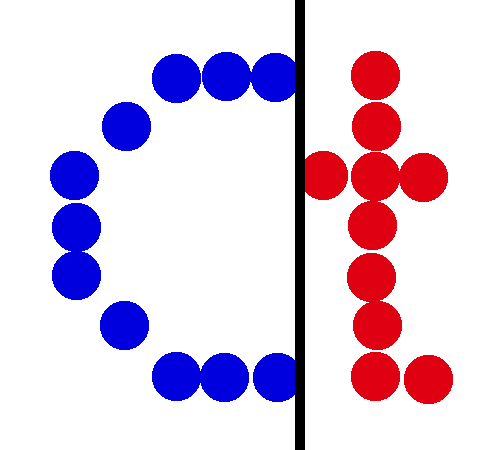
\includegraphics[width=150px]{10x9_Ct_split.png}
      \begin{alertblock}{}
            \begin{center}
                  \textbf{\Large Correctement détecté comme deux lettres}
            \end{center}
      \end{alertblock}
\end{frame}

\begin{frame}
\frametitle{OCR maison : séparation des caractères }
    \setbeamercolor{block body alerted}{fg=white,bg=blue}   
       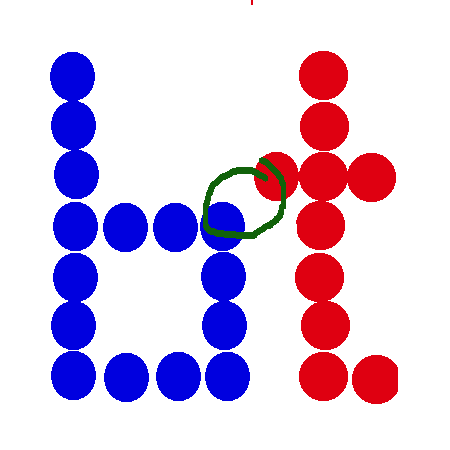
\includegraphics[width=120px]{9x9_bt_conflit.png}
      \begin{alertblock}{}
            \begin{center}
                  \textbf{\Large Ces deux caractères sont vus comme une seule lettre (à cause du pixel voisin en diagonale)}
            \end{center}
      \end{alertblock}

On pourrait relaxer les contraintes, ou redécouper un caractère trop large, ou incohérent après OCR. A voir plus tard.

\end{frame}

\begin{frame}
\frametitle{OCR maison : Reconnaître le caractère }
    \setbeamercolor{block body alerted}{fg=white,bg=blue}   
      \begin{alertblock}{}
            \begin{center}
                  \textbf{\Large Les méthodes dépendent du contexte}
            \end{center}
            \begin{itemize}
            \item pour un caractère isolé
            \item avec une connaissance typographique (on connaît la police)
            \item en utilisant des informations venant des caractères précédents
            \end{itemize}
      \end{alertblock}
\end{frame}


\begin{frame}
\frametitle{OCR maison : Reconnaître le caractère }
    \setbeamercolor{block body alerted}{fg=white,bg=blue}   
       \includesvg[width=350px]{Typography_Line_Terms}
      \begin{alertblock}{}
            \begin{center}
                  \textbf{\Large Un peu de vocabulaire}
            \end{center}
      \end{alertblock}
\end{frame}



\end{document}
